\documentclass[10pt,a4paper,twoside]{article}
\usepackage[a4paper,top=20mm,bottom=20mm,outer=5cm]{geometry}
\usepackage[utf8]{inputenc}
\usepackage[english]{babel}
\usepackage{graphicx}
%\usepackage{hyperref}
\usepackage{amsmath}
%\usepackage{cleveref}
\usepackage{natbib}
\bibliographystyle{abbrvnat}
\setcitestyle{authoryear}

\title{Project Machine Learning\\--- Milestone 1 ---}

%%%%%%%%%%%%%%%%%%%%%%%%%%%%%%%%%%%%%%%
%                                     %
%   EVERYTHING BELOW CAN BE CHANGED   %
%                                     %
%%%%%%%%%%%%%%%%%%%%%%%%%%%%%%%%%%%%%%%

\author{Konstantin Ausborn, Timon Palm, Marco Rosinus Serrano}
\date{\today}

% our own packages
\usepackage{acronym}
\usepackage{wrapfig}
\usepackage{listings}
\usepackage{float}
\usepackage{hyperref}
\usepackage{cleveref}

% acronyms
\acrodef{ae}[AE]{Autoencoder}
\acrodef{vae}[VAE]{Variational Autoencoder}
\acrodef{vq}[VQ-VAE]{Vector Quantized Variatonal Autoencoder}
\acrodef{gan}[GAN]{Generative Adversarial Networks}
\acrodef{dnn}[DNN]{Deep Neural Networks}
\acrodef{bpp}{bits per pixel}
\acrodef{mse}[MSE]{Mean Squared Error}
\acrodef{psnr}[PSNR]{Peak Signal to Noise Ratio}
\acrodef{nll}[NLL]{Negative Log Likelihood}
\acrodef{fid}[FID]{Fréchet Inception Distance}
\acrodef{ssim}[SSIM]{Structural Similarity Index Measure}
\acrodef{ilsvrc}[ILSVRC]{ImageNet Large Scale Visual Recognition Challenge 2012}
\acrodef{ml}[ML]{Machine Learning}
\acrodef{cnn}[CNN]{Convolutional Neural Network}
\acrodef{cifar}{CIFAR-10}

\begin{document}
    \maketitle
    \section{Introduction}\label{sec:introduction}
    
In the course of this machine learning project, we aim to implement a Vector-Quantized Variational Autoencoder (VQ-VAE)~\cite{vqvae} and to reproduce their results on the ImageNet and CIFAR-10 datasets.

In the first milestone, we focus on data preprocessing and the implementation of a baseline method for subsequent comparison.
This section will provide an overview of the datasets we will use, the preprocessing steps applied, and the baseline method we will implement. Additionally, we will outline the evaluation metrics that will be used to compare the performance of our VQ-VAE model with the baseline method.

Upon examining the ImageNet dataset, we found that it contains images with highly irregular resolutions, including some very small images, which was unexpected.
As a result, we performed additional data cleaning by removing images that were excessively small.
    \section{Datasets}\label{sec:datasets}
    The original \ac{vq} paper~\cite{vqvae} trained their model on three image datasets: \textit{ImageNet}, \textit{CIFAR-10}
, and video frames from \textit{DeepMind Lab}.
For this project, we will follow the same approach and train our \ac{vq} model on the ImageNet and CIFAR-10 datasets.

Image generation is an unsupervised learning task and therefore does not require labeled data.
Potentially, any kind of image data could be used for training and testing.
However, the quality of the generated
images is highly dependent on
the quality and diversity of the training data.

Further feature extraction methods are not necessary for the image generation task, as \ac{vq} works directly on pixel
values.
Image pixels are numerical values with a spatial correlation that \ac{vq} leverage.
\ac{vq} follows the Encoder-Decoder structure, learning a compressed representation of the input image in latent space.
Thus, \ac{vq} itself can be seen as a feature extraction/compression method.

ImageNet and CIFAR-10 are among the most common image datasets used in machine learning.
While they were originally designed for image classification and detection tasks, their utility extends beyond
these applications; by discarding the labels, they can also be leveraged for image generation tasks.
An overview of these two datasets is provided in Table~\ref{tab:datasets}

\subsection{ImageNet}\label{subsec:imagenet}
Upon examining the ImageNet dataset, we found that it contains images with highly irregular resolutions, including some
very small images, which was unexpected.
As a result, we performed additional data cleaning by removing images that were excessively small.

The full ImageNet dataset consists of 14.197.122 hand-labeled photographs collected from flickr and other search engines
~\cite{ILSVRC15,imagenet_breakdown}.

The images are distributed over 21841 \textit{synonym sets} from the \textit{WordNet}~\cite{wordnet} hierarchy,
pursuing to cover most nouns in the English language~\cite{imagenet_breakdown}.

When talking about ImageNet, most authors refer to the
\textit{ImageNet Large Scale Visual Recognition Challenge 2012} (ILSVRC) dataset~\cite{ILSVRC15},
which is a subset of the full dataset.
Hereinafter, we will refer to the ILSVRC 2012 dataset as ImageNet if not stated otherwise.

The ILSVRC set contains 1.281.167 unique labeled training images and 100.000 labeled test images distributed over 1000
classes.

ILSVRC was created as a computer vision benchmark.
It therefore additionally contains 50.000 validation images without labels, which we will not consider.
Three key computer vision tasks are benchmarked by the ILSVRC dataset: object classification, object localization and
object detection.
They address three fundamental computer vision questions: \textit{What is in the image?}, \textit{Where is it?} and
\textit{How many are there?}.

ImageNet is a supervised learning dataset with class id and bounding box annotations.
Though, it can also be used for unsupervised learning tasks like image generation, image compression or image denoising.

The collected images neither contain missing values nor duplicates and every image belongs to exactly one class.

The ImageNet dataset is designed to capture a diverse range of real-world scenarios across eight dimensions, as
illustrated in Figure~\ref{fig:imnet_dimensions} from~\cite{imagenet_breakdown}.
These dimensions include object scale (ranging from small to large objects), the number of instances (from few to many
objects present in an image), as well as variations in color and shape distinctiveness.

\begin{figure}
    \centering
    \includegraphics[width=\textwidth]{../../sample_images/imnet_dimension}
    \caption{Eight diversity dimensions of the ImageNet dataset~\cite{imagenet_breakdown}}
    \label{fig:imnet_dimensions}
\end{figure}

The majority of classes contain 1300 examples, though it is not entirely balanced across the classes.
In fact, some classes have fewer examples, as shown in Figure~\ref{fig:imnet_dist}.
Among the classes with the lowest number of images are \textit{"black-and-tan coonhound"}, \textit{"otterhound"} and
\textit{"English foxhound"} with 732, 738 and 754 samples, respectively.
Note: These are different dog breeds

A class disbalance in the training data can lead to a bias in the resulting model.
We access the class distribution in the ImageNet dataset more or less balanced, as most classes contain 1300 images.
The classes with fewer examples are still represented by a reasonable number of images.
Moreover, the number samples for different dog breeds for instance might be lower, but still the number of dog images is fairly high.
Our goal for this project might not be to generate
images of different dog breeds, just a dog image suffices.

Upon examining the plethora of different shapes present in the ImageNet dataset, we found that the images have highly
irregular resolutions.
The resolutions range from 8x10 pixels to 9331x6530 pixels with a mean resolution of 471.7x404.7 pixels, as shown in
Figure~\ref{fig:imnet_sizes_err}.
The histogram in Figure~\ref{fig:imnet_sizes_hist} illustrates the distribution of image resolutions in the dataset.

As to be seen in figure~\ref{fig:optimal_resolution}
, some images have a very irregular ratio, which imposes a challenge for resizing.
Very small images do not contain enough information, which when upscaled, result in a blurry image (illustrated in
figure~\ref{fig:small_image}).
We decided to remove such images and restrict the dataset to a minimum image size of 32x32 pixels.

\begin{figure}
    \centering
    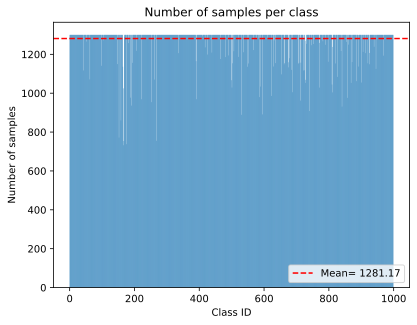
\includegraphics[width=\textwidth]{../../sample_images/imagenet_dist}
    \caption{Distribution of images per class in the ImageNet dataset}
    \label{fig:imnet_dist}
\end{figure}

\subsubsection{Preprocessing}
In order to train the \ac{vq} on the ImageNet dataset, we will do the following preprocessing steps.

\begin{itemize}
    \item \textbf{Image Resizing:}
    For training and testing, we resize all images to 128x128 pixels, similar to the paper~\cite{vqvae}.
    \item By virtue of the \ac{vq} architecture, a latent space of 32x32x1 pixel is implied.
    There are different ways one can resize an image.
    \item We use a composition of random cropping to extract a square image
    and resize it to 128x128 pixels with the TorchVision
    \texttt{v2.RandomResizedCrop(size, scale, ratio, antialias=True)}.
    \item We set \texttt{scale=(0.2, 1.0)} and \texttt{ratio=1} to crop a square image with a sufficient area in
    relation to the original image.\\
    We keep the standard \textit{Bilinear interpolation} for resizing and set \texttt{antialias=True}
    to reduce aliasing artifacts.

    \item \textbf{MinMax Normalizing:}
    The pixel values of the images are in the range of 0 to 255.
    We scale them to the range of 0 to 1 by dividing them by 255.
    When input features have different scales, normalizing is a necessity for stable convergence.
    In the case of images, the pixel values are already in the same range, but normalizing them will help to stabilize the training
    process.

    \item \textbf{Standardization:}
    Standardizing is a common step in machine learning and also often used for ImageNet, e.g.\ for training ResNet
    ~\cite{resnet}.
    It is also part of the standard TensorFlow and PyTorch preprocessing pipeline for ImageNet. \\
    We standardize the images with the mean $\mu = (0.485, 0.456, 0.406)$ and standard deviation
    $\sigma = (0.229, 0.224, 0.225)$ of ImageNet for the three color channels, respectively.

\end{itemize}

Example images from ImageNet dataset after preprocessing are depicted in figure~\ref{fig:imnet_example_normalized}.

\subsection{CIFAR-10}\label{subsec:cifar-10}
CIFAR-10~\cite{cifar10} is another popular image classification dataset, as well as the larger version CIFAR-100.
CIFAR-10 consists of 60.000
32x32 pixel images, which are distributed over 10 classes.
The dataset is split into 50.000 training images and 10.000 test images.
The classes are mutually exclusive, so each image belongs to exactly one class.
The classes are: \textit{airplane, automobile, bird, cat, deer, dog, frog, horse, ship, truck}

The train set contains exactly 5000 images per class, while the test set contains 1000 images per class.
No image belongs to more than one class and there are no missing values or duplicates in the dataset.

\subsubsection{Preprocessing}
As the images in the CIFAR-10 dataset are already 32x32 pixels, we do not need to resize them.
Hence, we will only apply MinMax Normalizing and potentially Standardizing, same as for the ImageNet data.

Example images from the CIFAR-10 dataset are shown in figure~\ref{fig:cifar10_example_normalized}.

\begin{table}[]
    \begin{tabular}{lllll}
        Dataset  & \# train images & \# test images & \# classes & image size           \\ \hline \hline
        ILSVRC   & 1.281.167       & 100.000        & 1000       & 8--10px - 9331x6530px \\
        CIFAR-10 & 50.000          & 10.000         & 10         & 32x32px              \\ \hline \hline
    \end{tabular}
    \caption{Datset overview: ImageNet and CIFAR-10}
    \label{tab:datasets}
\end{table}

    \section{Evaluation Metrics}\label{sec:evaluation-metrics}
    The metrics usable for the tasks described in Section~\ref{sec:introduction} are manifold.
As not all metrics are suitable for all the work done by the model.
We therefore split this section into two subsections.

\subsection{Compression}\label{subsec:compression}
For compression, the most straightforward metric is to measure the reduction of memory required to
store the data.
To normalize over image resolution, we choose to evaluate the \ac{bpp}.

The second, and less objective measure, is image similarity after reconstruction.
While the \ac{mse} and by transfer \ac{psnr} describe pixel-wise similarity very well, it is not
always optimal to judge perceived similarity for humans, as can be seen in Figure~\ref{fig:mse_ssim}.

\[
\text{MSE} = \frac{1}{n} \sum_{i=1}^{n} (y_i - x_i)^2 \quad \quad \text{PSNR} = 10 \cdot \log_{10} \left( \frac{\text{MAX$^2$}}{\text{MSE}} \right)
\]
where $\text{MAX}$ is the maximum possible pixel value (255 for our 8-bit images).

\begin{figure}[ht]
    \centering
    \includegraphics[width=0.6\textwidth]{images/ssim_mse}
    \caption{Two images with the same \ac{mse} with reference from~\cite{scikit-ssim}}
    \label{fig:mse_ssim}
\end{figure}

To overcome these limitations we use the \ac{ssim}, a metric working under the assumption that human visual
perception is highly adapted for extracting structural information from a scene~\cite{ssim}.

\[
\text{SSIM}(x, y) = \frac{(2\mu_x \mu_y + C_1)(2\sigma_{xy} + C_2)}{(\mu_x^2 + \mu_y^2 + C_1)(\sigma_x^2 + \sigma_y^2 + C_2)}
\]
$\text{where } C_1 \text{ and } C_2 \text{ are constants to avoid dividing by zero.}$


Even though this analysis favours \ac{ssim}, we use \ac{mse} as our loss function for our baseline models,
since the \ac{vq} implementation we plan to replicate does the same, and we want to maximize comparability.
We use \ac{ssim} for result evaluation, and add \ac{psnr} values for further experiments.

\subsection{Image Generation}\label{subsec:image-generation}
An important metric in Image Generation is the \ac{nll} normalized to the amount of pixels (dimensions) in an image, given in bits/dim.
It is used to argue about the strong performance of the \ac{vq} in the paper.
A lower number indicates a higher likelihood of generating the test data given our model.
The bits/dim number is rooted in information theory, and describes the average number of bits required to
compress the test data with the entropy coding scheme that is optimal for a model~\cite{shannon}.

The \ac{fid}, introduced by~\cite{fid}, is another interesting metric.
It compares the distribution of features of a generator with that of real images via a network trained on a big
dataset, often also imagenet.

Another criterion not to be left out is the classic human turing test, as in evaluating the images by hand.
Even though this is not scalable, it is the ultimate classifier for human perception, and can be a good starting
point.

For metrics we decided not to use: The paper introducing \ac{fid} shows it is more consistent than the earlier and
similar inception score, so we excluded the latter.
Research advises against using Parzen Window Estimates~\cite{note_on_eval}, so we avoided them as well.

Since we have not yet implemented any image generation functionality, the value of these metrics remains to be evaluated.

TODO: INTRODUCE FORMULAS FOR THE CRITERIONS

    \section{Baseline Methods}\label{sec:baseline-methods}
    The \ac{vq} described in the paper both learns useful and compact, discrete representations of real world data,
and generates new samples in this representation space and decoding them back to the original data space.
A good baseline would align to this collection of tasks as close as possible.

While there exist multiple machine learning approaches with a setup similar to that of the \ac{vq}
i.e.\ generative models with latent representations such as \ac{gan}, differences in the details make these hard to
compare against each other.
When sticking to the example of \ac{gan} as described by~\cite{gan}, one key difference is that similar to the
\ac{vq} after training the PixelCNN, the latents represent a distribution that is close to that of the training
data, but can not be created by encoding real world data.

\subsection{Autoencoder}\label{subsec:autoencoder}
Since it is the original model that the non-quantized \ac{vae} is based on, which in turn later was developed into the
\ac{vq} and because it also fulfils our requirement of sufficient simplicity, we chose a basic \ac{ae} as our general
baseline method.

A very basic \ac{ae} as described by~\cite{autoenc} and illustrated in Figure~\ref{fig:ae}, is a neural
network that is fed
the
original data, in our case the
image, and then compresses the data down to a lower dimension using one or more hidden and fully connected layers,
the encoding stage.
The result of this encoding stage is fed into a latent layer, whose dimensions decide the size of the compressed
representation.
The output of this latent layer, the actual latent, is than upsampled by a decoding stage, which follows an inverted
structure of the encoding stage.
The output of the net, the reconstruction, is now of the same shape as the input data and can be directly compared
to it.

The model can be trained by applying gradient descent on some form of cost function that describes reconstruction error
like \ac{mse}, theoretically pushing the network to encode the information most important to deconstruction in the
latent.

The similarities to \ac{vq} allow for very comparable results, since the \ac{ae} can be tuned to be very
close in size, training and inference cost.
During implementation of the \ac{ae} baseline, we adhere to the same architecture as the \ac{vq} wherever possible,
exchanging the fully connected layers of the standard \ac{ae} with the downsampling layers and
residual blocks from the \ac{vq} implementation in our reference paper.
This will likely increase its power significantly, as convolutional \ac{ae} have been shown to be superior to the
basic feed-forward \ac{ae} on the realm of image reconstruction by~\cite{convae}.

\begin{figure}[H]
    \centering
    \includegraphics[width=0.7\textwidth]{images/ae}
    \caption{Illustration of a basic \ac{ae} architecture from~\cite{ae_pic}}
    \label{fig:ae}
\end{figure}

\subsection{Variational AE}\label{subsec:variational-ae}
Examining the differences between the different evolutionary steps towards the \ac{vq} could prove to be valuable
for our understanding of its performance.
Therefore, we also implement a \ac{vae}, which substantially differs from the \ac{ae} in the way that latents are
generated.
When constructing the neural network, we follow the same paradigm as with the \ac{ae} before, using the same
encoding and decoding layers as far as possible.
The important difference of the VAE is that its encoder outputs a random variable
$\boldsymbol{\hat{z}} \sim \mathcal{N}(\boldsymbol{\mu_\theta}, \text{diag}
(\boldsymbol{\sigma_\theta}))$. $\boldsymbol{\hat{z}}$ is obtained using the
reparameterization trick, which consists in sampling $\boldsymbol{z}
\sim \mathcal{N}(0, I)$ and then computing $\boldsymbol{\hat{z}} =
\boldsymbol{\mu_\theta} + \boldsymbol{z} \odot \boldsymbol{\sigma_\theta}$.
$\boldsymbol{\mu_\theta}$ and $\boldsymbol{\sigma_\theta}$ are deterministic
outputs of the last convolutional layer of the \ac{vae} encoder.
This allows to optimize the model using the ELBO loss which in turn enables us to not only
reconstruct the input, but to learn a posterior distribution $p(x|z)$ while
the encoder $q(z|x)$ tries to be as close as possible to $p(z)$.
Thus enabling us to generate new dataset samples by sampling $z \sim p(z)$ and then feeding
it through the decoder.

\textbf{A Note on Overfitting}
Overfitting refers to the phenomenon where a model starts to memorize the training data instead of learning useful
features from the training data that generalize well to unseen data as is the goal.

While theoretically, this may very well be an issue with \ac{ae} and \ac{vae}, we have not experienced this happening
yet with either when training with adequate training-set sizes.
This is very likely due to the large dataset size and the inductive bias of the convolution operation~\cite{citationNeeded}.

\subsection{Non-ML Baseline: JPEG}\label{subsec:jpeg}
While much of the current work in realistic high resolution image generation is based on \ac{dnn}~\cite{citationNeeded},
the field of image compression is well researched both in-, and outside deep architectures~\cite{compression},
and non-ML approaches are still dominant on the web as can be seen in Figure~\ref{fig:file_formats}.
To represent this, we also use the popular JPEG format for comparisons against our lossy compression schemes.

\begin{figure}[H]
    \centering
    \includegraphics[width=0.5\textwidth]{images/formats}
    \caption{Percentages of websites using various image file formats~\cite{img_file_format}}
    \label{fig:file_formats}
\end{figure}
    \section{Discussion}\label{sec:discussion}
    The following sections will discuss the results of our baseline experiments, further ideas for the project, and real-world applications of the project.

\subsection{Baseline Experiments}\label{subsec:baseline-results}
    We present some results of our baseline training runs. We did an examplarily training for 10 epochs on a subset of ImageNet to see that it converges. The subset contained 100.000 images with 1000 samples per class. See ... for the full configuration details.
    
    \subsubsection{Autoencoder}\label{subsubsec:autoencoder}
        We were able to show that our implementation of an \ac{ae} is able to reconstruct images from the ImageNet dataset. W

        For this trainig, we used a latent dimension of 32x32x2 pixels, which means 4 bits per pixel for an 128x128x3 input images. That is a compression rate of 4,7 \% compared to the original image size.

        We are surprised by the results of our basic \ac{ae} and its capability to reconstruct images. Even with a realitively small latent dimension and only 10 epochs of training it is able to reconstruct images with a satifiying human percetiple quality.
        
        

\subsubsection{Class Differences}\label{subsubsec:class-differences}
\subsection{Further Ideas for the Project}\label{subsec:further-ideas}
\subsection{Real World Use of the Datasets}\label{subsec:real-world-applications}
\ac{cifar} and ImageNet have been around for one and a half decades.
Overall, their use-case has shifted from being the cutting edge datasets to train on to
more of a dataset for experiments and benchmarks.

The outstanding status of ImageNet in its early days gets apparent when looking at AlexNet~\cite{AlexNet}.
The paper on training a \ac{cnn} on ImageNet with \ac{GPU}s has been cited a staggering 166 thousand times as of the
time of this report and is seen as one the starting points of the rise of \ac{dnn}.

Today, the newest (text-based) image generation networks use much bigger datasets, with sample sizes stretching into
the billions.
One prominent example of such datasets is LAION-5B described by~\cite{laion5b}, which is for example used by Stable
Diffusion based on the work of~\cite{stable_diff}.
When examining this paper in greater detail, the continued relevance of ImageNet becomes clear.
First, the dataset is used to train experimental networks, which would be prohibitively expensive to train on larger,
modern datasets.
Furthermore, metrics like the \ac{fid}, also introduced in Section~\ref{sec:evaluation-metrics}, are used calculated on
ImageNet, further underscoring its importance for research.

Similar observations can be made for \ac{cifar-10}, but its limited resolution makes it less suitable for
benchmarking modern approaches to image generation.

Given these observations, while we anticipate producing some convincing results with our final model,
we do not expect to match the visual fidelity achieved by state-of-the-art image generation models.


\vskip 1em
\textbf{A Note on Overfitting:}
Overfitting refers to the phenomenon where a model starts to memorize the training data instead of learning useful
features, in turn not generalizing well to unseen data.

While theoretically, this may very well be an issue with \ac{ae} and \ac{vae}, we have not experienced this happening
yet with either when training with adequate training-set sizes.
This is likely due to the large dataset sizes we use and the inductive bias of the convolution operation~
\cite{citationNeeded}.
    \bibliography{bibliography}
    \section{Appendix}\label{sec:appendix}
    \begin{figure}
        \centering
        \includegraphics[width=0.5\textwidth]{../../sample_images/imagenet_unnormalized}
        \caption{Example images from the ImageNet dataset randomly cropped and resized to 128x128 pixels and standardized}
        \label{fig:imnet_example_normalized}
    \end{figure}

    \begin{figure}
        \centering
        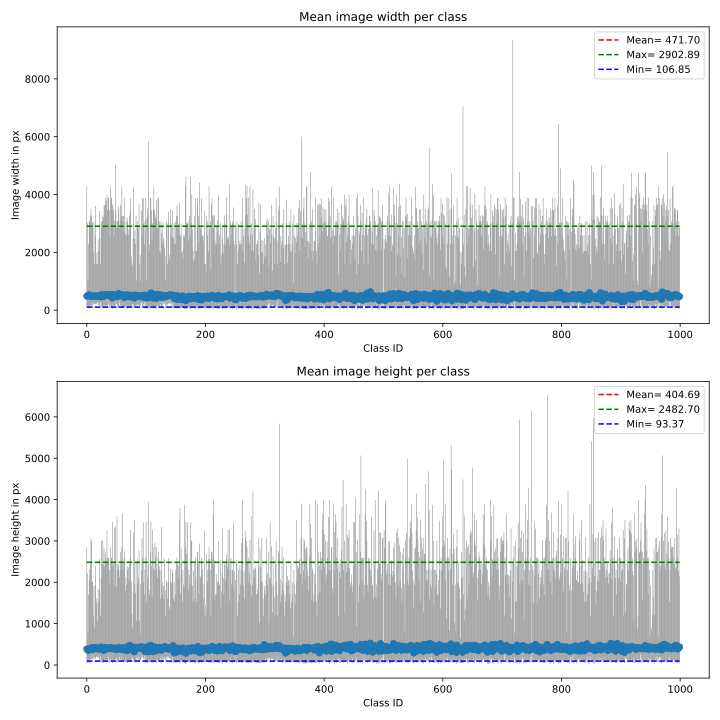
\includegraphics[width=0.5\textwidth]{../../sample_images/imagenet_sizes_errorbar}
        \caption{Image resolution deviations in the ImageNet dataset across classes}
        \label{fig:imnet_sizes_err}
    \end{figure}

    \begin{figure}
        \centering
        \includegraphics[width=0.5\textwidth]{../../sample_images/imagenet_sizes_histogram}
        \caption{Histogram of image resolutions in the ImageNet dataset}
        \label{fig:imnet_sizes_hist}
    \end{figure}

    \begin{figure}
        \centering
        \includegraphics[width=0.5\textwidth]{../../sample_images/cifar_rbatch}
        \caption{Example images from the CIFAR-10 dataset standardized}
        \label{fig:cifar10_example_normalized}
    \end{figure}

    \begin{figure}
        \centering
        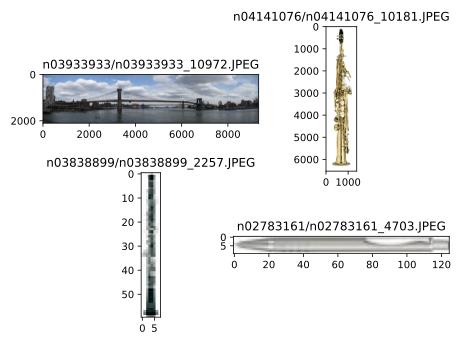
\includegraphics[width=0.5\textwidth]{../../sample_images/optima_shape_examples}
        \caption{Example images from the ImageNet dataset with very unregular resolution ratios}
        \label{fig:optimal_resolution}
    \end{figure}

    \begin{figure}
        \centering
        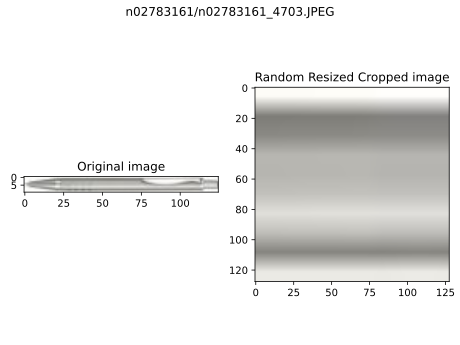
\includegraphics[width=0.5\textwidth]{../../sample_images/random_resized_crop_small}
        \caption{Example image from the ImageNet dataset that is too small}
        \label{fig:small_image}
    \end{figure}
\end{document}
